Alla luce di quanto scritto finora, una possibile applicazione della tecnologia si può individuare nell'e-voting. Nei sistemi di voto attualmente in uso, la correttezza del voto e l’anonimato del votante sono totalmente affidati al controllo di un ente o di un sistema centrale in cui si ha fiducia come può essere lo stato o l'organo che indice la votazione. Questo vincola gli eleggibili e gli elettori ad una mancanza di trasparenza finora ritenuta inevitabile, e il sistema elettorale a dover investire risorse considerevoli nel gestire la votazione a partire da quando viene indetta fino al termine degli scrutini. L’avvento della tecnologia Blockchain permette un cambio di paradigma in favore di sistemi decentralizzati e trasparenti in cui non sia necessario riporre fiducia nell’operato di alcuno degli agenti coinvolti. Si propone quindi un modello che permetta di applicare queste caratteristiche desiderabili ad una votazione elettronica.

\section{Tecnologie e algoritmi utilizzati}
	\subsection{Hyperledger Fabric v.1.0}
		Hyperledger è un progetto collaborativo della Linux Foundation che mira a creare un framework open source per lo sviluppo di sistemi Blockchain in ambito aziendale. Fabric è uno dei sottoprogetti che fanno parte di Hyperledger, in particolare rappresenta il principale contributo di IBM alla causa. Nella visione di Hyperledger Fabric un sistema Blockchain aziendale deve essere basato su di un'architettura modulare in cui i diversi elementi, come algoritmi di consenso, sistema di verifica delle identità, protocolli di cifratura o tipo di database ausiliari, siano intercambiabili e sostituibili liberamente. Permette anche lo sviluppo di smart contract, qui chiamati chaincode, attraverso l'uso di un qualsiasi linguaggio di programmazione: caratteristica che lo rende estremamente più flessibile del limitato set di istruzioni previsto da Bitcoin o dal linguaggio dedicato sviluppato da Ethereum. Per fare ciò l'esecuzione dei chaincode è isolata in un container dedicato, creato attraverso Docker, contenente un sistema operativo sicuro, il linguaggio del chaincode e gli SDK che permettono di interfacciarsi con il sistema. Fabric è un sistema permissioned, tutti i partecipanti sono tenuti ad autenticarsi attraverso un servizio dedicato (anche questo intercambiabile) per avere accesso alla rete. 
		\subsubsection{Componenti di Fabric}
			\begin{itemize}
				\item \textbf{Client}: sono gli enti partecipanti alla rete che invocano un chaincode o propongono una transazione. Rappresentano gli utenti finali, non mantengono una copia della blockchain ma devono connettersi con un peer per interagire con il sistema;
				\item \textbf{Peer}: sono gli enti che effettuano le transazioni e mantengono il database condiviso e la blockchain. I peer sono coordinati dall'orderer secondo delle policy specificate a priori;
				\item \textbf{Orderer}: è l'ente (eventualmente distribuito) che sovrintende alla comunicazione tra i nodi della rete. Fornisce garanzie di consegna dei messaggi immessi nella rete, tra cui le proposte di transazione da parte dei peer. È il responsabile del consenso all'interno del sistema distribuito;
				\item \textbf{Membership services}: sono l'astrazione di tutti i meccanismi crittografici e i protocolli che lavorano alla validazione dei certificati e al riconoscimento degli utenti; 
				\item \textbf{Organizzazioni}: rappresentano ciascuna entità distinta che possiede un certificato univoco per la rete. I nodi come i peer o i client devono essere legati ad un'organizzazione per poter essere riconosciuti e autenticati;
				\item \textbf{Channel}: è l'overlay della blockchain privata di Hyperledger. Ciascun canale ha un registro specifico, condiviso tra i peer registrati al canale, e ciascun ente coinvolto nella transazione deve essere autenticato ad uno specifico channel affinché questa abbia luogo;
				\item \textbf{State}: abbreviazione per "State Database", è il database in cui è salvato lo stato attuale del sistema per effettuare query sul registro in maniera efficiente. È modellato come un database chiave/valore con versionamento. Può essere completamente ricostruito dalla storia delle transazioni salvata in blockchain, il che ne garantisce il controllo sull'affidabilità;
				\item \textbf{Chaincode}: è il nome dato ai programmi salvati nella blockchain di Hyperledger. Sono invocati dalle transazioni, e possono inizializzare componenti nello state o modificarli. La loro esecuzione avviene in un container Docker isolato per garantirne la riservatezza. Incapsula la componente di business logic del sistema, ha corrispondenza diretta con quelli che in altri sistemi basati su Blockchain vengono chiamati \emph{smart contract}.
				\item \textbf{Transazioni}: sono la rappresentazione di ogni azione effettuata sul registro. Possono essere \emph{deploy transactions} che creano nuovo chaincode e lo ``installano" in un canale oppure \emph{invoke transactions} che invocano una funzione presente in un chaincode installato per effettuare letture o modifiche al ledger. Ciascuna transazione deve essere approvata e gestita dall'orderer, e viene registrata nella blockchain per la futura tracciabilità.
			\end{itemize}
		
	\subsection{Ring signature}
		Una ring signature, o firma ad anello, è un tipo di firma digitale legata ad un gruppo di utenti ciascuno in possesso di una chiave. Questo tipo di firma permette di verificare che l'autore appartiene a quel dato gruppo di utenti rendendo però computazionalmente infattibile determinare quale specifico utente esso sia. Riporto di seguito (tradotta) una possibile definizione formale \cite{ring_signature}: \\
		Si supponga che un gruppo di entità possieda le coppie di chiavi pubbliche/private 


\section{Architettura}
	Il sistema si articola in due blockchain separate, la blockchain di firma e la blockchain di voto (da ora rispettivamente Signature chain o SC e Vote chain o VC). Le due chain sono isolate, per garantire la non collegabilità del voto al votante in fase di scrutinio.
	Le due chain hanno scopi diversi: SC assicura che il voto avvenga in maniera controllata e abilita al voto il client, inoltre contiene le informazioni per dividere in raggruppamenti i votanti similmente a quanto avviene con le sezioni elettorali; VC raccoglie i voti e li registra per effettuare poi il conteggio, ma deve garantire l’anonimato del votante.
	
	\subsection{Preparazione}
		Viene indetta una votazione. Si prevede che l'architettura sia già predisposta, in particolare devono essere noti ed affidabili, completi di chiavi pubbliche:
		\begin{itemize}
			\item L'elenco dei votanti;
			\item L'elenco dei peer;
			\item L'elenco degli indirizzi dei candidati per la Vote chain;
			\item L'elenco dei programmi client verificati.
		\end{itemize}
		\subsubsection{Inizializzazione della Signature chain}
			La SC viene predisposta con il chaincode che permette al client di interrogare la chain per conoscere le chiavi pubbliche dei votanti inseriti nello stesso raggruppamento, registrando contemporaneamente la propria firma. I dati sui raggruppamenti dei votanti sono inseriti nella SC. Questa dovrà essere accessibile solamente ai peer deputati al controllo della votazione, a causa della riservatezza delle informazioni sui raggruppamenti.
		\subsubsection{Inizializzazione della Vote chain}
			La VC contiene inizialmente delle transazioni che registrano l'associazione di ogni indirizzo numerico ad un nome intelligibile del candidato corrispondente, i saldi dei voti dei candidati inizializzati a 0 e il chaincode necessario al client per incrementare di 1 il saldo del candidato scelto. Un altro chaincode utile è quello che permette ai peer di ricevere il conteggio finale e quindi l'esito della votazione, così come il chaincode che permette ad un servizio web di interrogare la blockchain e rendere pubblici i dati in essa contenuti per permettere al votante la verifica del voto espresso.
	
	\subsection{Workflow di una votazione}
		\begin{figure}[ht]
			\centering
			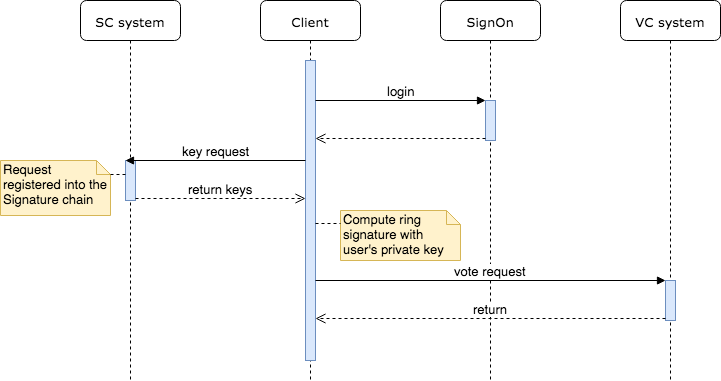
\includegraphics[width=\textwidth]{voting_workflow.png}
			\caption{Workflow della votazione}
			\label{fig:voting_workflow}
		\end{figure}
		Il diagramma in \hyperref[fig:voting_workflow]{figura \ref*{fig:voting_workflow}} illustra il workflow tipico di una votazione.
		\subsubsection{Signature chain: Firma del registro votanti}
			Il client autentica l'utente attraverso un \hyperref[subsec:personalita_voto]{sign-on affidabile}. I controlli di accesso possono essere rinforzati o meno da \hyperref[subsec:liberta_voto]{altri passaggi} affidati a sistemi di intelligenza artificiale o al controllo di un operatore. A utente autenticato, il client invoca il chaincode di query su SC ed ottiene l'elenco delle chiavi pubbliche del suo raggruppamento. Questa richiesta viene registrata in blockchain, per assicurarsi che lo stesso utente non possa ripetere la procedura di voto due volte.
			
		\subsubsection{Vote chain: In cabina elettorale}
			Il client si trova ora in possesso delle chiavi pubbliche della sua sezione. In locale permette al votante di esprimere la propria preferenza di voto e richiede la transazione corrispondente nella VC firmandola con la ring signature del proprio raggruppamento.
			La votazione è ora conclusa.
		
		\subsubsection{Scrutinio e verifica}
			Le operazioni di scrutinio e verifica possono ora essere completamente automatizzate, facendo riferimento ad una base di dati sicura e virtualmente inalterabile come la blockchain.

\section{Analisi}
	In questa sezione si analizzano le scelte architetturali fatte argomentandole, concludendo con delle possibilità di miglioramento che si potranno presentare con l'avanzamento dello scenario tecnologico attuale.
	
	\subsection{Qualità del voto}
		Il voto è definito dall'art. 48 \cite{art48} della Costituzione Italiana come "personale ed eguale, libero e segreto".
		\subsubsection{Personalità}\label{subsec:personalita_voto}
			La personalità del voto, intesa come la necessità di esercitarlo di persona e non tramite terzi, è delegata in questa proposta al servizio di sign-on. Al momento attuale, è possibile fare affidamento su diversi sistemi di autenticazione: per il corretto funzionamento del sistema è previsto che ogni utente abbia una coppia di chiavi pubblica e privata distribuita precedentemente, sotto verifica di un operatore. Ad esempio, è possibile distribuire queste chiavi contestualmente alla consegna della tessera elettorale. La natura certificata di queste chiavi le rende ideali come metodo di autenticazione ma è possibile aggiungere ulteriori controlli come una verifica tramite dati biometrici.
		
		\subsubsection{Eguaglianza}
			L'eguaglianza del voto consiste nell'avere ogni voto lo stesso valore di tutti gli altri. Si articola nell'impedire, in particolare, il voto plurimo e il voto multiplo. Nel sistema proposto, il voto plurimo è scongiurato dal codice del chaincode della Vote chain, il quale permette solo incrementi unitari al saldo dei candidati. Uno scenario di voto multiplo è invece controllato dalla Signature chain e dalla struttura del client: è infatti indispensabile che la procedura di voto sia strettamente successiva alla procedura di firma in SC, e non invocabile in maniera indipendente. In tal modo è possibile garantire che una stessa persona non reiteri l'esecuzione del chaincode di voto. Pur ammettendo il caso in cui un attaccante riesca a violare il client, questo potrà reiterare voti firmati dalla stessa ring signature: un controllo automatico può facilmente accorgersi della non coerenza del numero di votanti nel raggruppamento e il numero di voti espressi dal raggruppamento, invalidando di fatto le transazioni ma mantenendo confinato l'evento disastroso: si possono applicare le procedure invocate attualmente qualora venissero riscontrate irregolarità che compromettano la validità dei voti di una sezione elettorale.
		
		\subsubsection{Libertà}\label{subsec:liberta_voto}
			La libertà del voto viene garantita dal negare la possibilità di voto qualora il votante fosse stato costretto con mezzi illeciti a esprimere una certa preferenza. Nel sistema di voto attuale è garantita dal controllo degli operatori di seggio. Nei sistemi di voto remoto l'argomento risulta spinoso: è infatti estremamente difficile stabilire una situazione di particolare pressione dell'elettore, o l'interferenza di esterni. Nel caso di voto elettronico, forzare il client ufficiale a poter essere installato solo su dispositivi muniti di telecamera frontale potrebbe risolvere il problema. Il controllo può essere svolto da appositi addetti eventualmente aiutati da un'intelligenza artificiale simile a quella utilizzata da Unilever \cite{ai_unilever} per i colloqui di lavoro. Questo non scongiura ogni possibile manipolazione, ma va evidenziato che il controllo sul sistema proposto non lo rende meno sicuro del sistema già in essere: permette anzi un livello di garanzia estremamente più alto di quello dei sistemi di voto per corrispondenza, già accettati in Italia in caso di votanti dall'estero e adottato in maniera diffusa in Svizzera.
		
		\subsubsection{Segretezza}
			La segretezza del voto nel sistema proposto ha come fulcro la completa separazione delle due blockchain. Affidando al client il compito di mantenere la continuità dell'operazione di voto, l'accoppiamento tra votante e voto espresso non può essere ricostruito con certezza in alcun modo. L'unica informazione che può trapelare riguarda il momento in cui viene registrata la votazione nelle due chain, tuttavia questa informazione è molto meno affidabile di quanto possa sembrare a causa della \href{sec:teorema_CAP}{consistenza eventuale} della blockchain. Sebbene qualche informazione trapeli, l'elevato numero di transazioni contemporanee previsto e l'incertezza nel determinare l'esatto momento di voto rende di fatto inservibili queste informazioni.
	
	
	\subsection{Necessità dei raggruppamenti}
		La suddivisione in sezioni elettorali è assolutamente necessaria nel sistema di voto attualmente adottato a causa di problemi logistici: è impensabile infatti raggruppare tutte le schede e svolgere un'unica operazione di scrutinio, soprattutto considerando il livello di sorveglianza che sarebbe richiesto in ogni momento dell'operazione. In un sistema automatico come quello proposto, esente da queste problematiche, sono stati introdotti raggruppamenti di elettori per differenti ragioni. In primo luogo, la complessità computazionale degli algoritmi più noti e affermati per la ring signature è lineare: questo preclude l'uso significativo di questa tecnologia (centrale nel modello proposto) per insiemi di chiavi sufficientemente grandi. In secondo luogo, nel caso un attacco permettesse di replicare lo stesso voto più volte la divisione in raggruppamenti permette di contenere i danni al solo raggruppamento interessato.
		È da sottolineare come, nel caso di un sistema elettronico, l'indipendenza dai problemi logistici dei sistemi tradizionali permetta di variare di volta in volta la composizione dei raggruppamenti, rendendo inutile qualsiasi informazione trapelata dalle votazioni precedenti. Questa è una condizione certamente più sicura di quella attuale, dove una semplice osservazione sul posto permette di identificare gli appartenenti a ciascuna sezione e far trapelare quindi informazioni (per quanto parziali) sulle preferenze di voto espresse: essendo i risultati delle votazioni per seggio pubblici, il trapelare di qualsiasi informazione sulla composizione del seggio è da considerarsi quantomeno indesiderato.
	
	\subsection{Prevedibili miglioramenti futuri al sistema}
		Al momento passaggi critici come l'autenticazione utente e il passaggio dalla SC alla VC devono essere svolti off-chain, ma future scoperte potrebbero aprire la strada verso implementazioni più complete.
		Portare l'autenticazione utente su Blockchain è un progetto che si lega con la creazione di un sistema di identità digitale decentralizzata. Immaginando un futuro (ad ora remoto) in cui siano disponibili documenti affidabili on-chain attraverso qualche tecnologia, l'autenticazione utente potrebbe svolgersi in questo modo guadagnando le caratteristiche di decentralità e sicurezza proprie della Blockchain. \\
		Più vicino alla situazione attuale è un meccanismo che permetta di abilitare alla votazione su VC direttamente da SC, senza rinunciare all'anonimato del votante. Al momento, ogni chaincode di Hyperledger è eseguito in un ambiente completamente isolato per ragioni di sicurezza. Sono già previste successive implementazioni che permettano a diversi chaincode di interagire tra di loro. Questo aprirebbe ad una modifica del sistema di voto proposto: sarebbe possibile implementare su VC un sistema di token: questi token sarebbero generati quando viene indetta la votazione in base al numero di aventi diritto al voto, e versati dai chaincode verso dei ``portafogli" temporanei da loro generati casualmente. Questi sarebbero poi passati al client già cifrati in maniera da mantenere chiunque, eccetto il software del chaincode, all'oscuro dell'accoppiamento votante-portafoglio. In questo modo sarebbe possibile prescindere dai raggruppamenti affidando la sicurezza del sistema unicamente alla solidità della Blockchain. L'aspetto negativo è che si perderebbe la capacità dei raggruppamenti di confinare un eventuale attaccante.